% --------------------------------------------------------------
% This is all preamble
% --------------------------------------------------------------
 
\documentclass[10pt]{article}


% Basic Packages for Encoding (Input AND Output) and Langauge Support
\usepackage[utf8]{inputenc}
\usepackage[T1]{fontenc}
\usepackage[french]{babel}

% Change Layout with a User-Friendly Interface
\usepackage[margin=1in]{geometry} 

% Include Pictures with a User-Friendly Interface
\usepackage{graphicx}
\graphicspath{ {./images/statistics_and_probability/} }
\usepackage{float}

% Extended Math Support from the Famous 'American Mathematical Society'
\usepackage{amsmath,amsthm,amssymb}

% Section title formatting
\usepackage{titlesec}

\titleformat{\section}
            {\normalfont\scshape}{\thesection}{1em}{}

\newcommand{\N}{\mathbb{N}}
\newcommand{\Z}{\mathbb{Z}}

%Numbered Questions 
\newcounter{question}
\newenvironment{question}
               {\refstepcounter{question}\par\medskip\noindent\textbf{Q~\thequestion.}\par \noindent \rmfamily}
               {\medskip}
 
\begin{document}
 
% --------------------------------------------------------------
%                        Actual content
% --------------------------------------------------------------

\title{Exercices de révision: Statistiques et probabilité}
\author{Annie B. \thanks{Les questions sont tirées des examens de l’IB de 2018, 2012, 2011, 2010, 2007}}
\date{\today}
\maketitle

\section*{\emph{Calculatrice Graphique Non Permise}}

\begin{question}
  \hspace*{\fill} [Note maximale: 6]\par
  \noindent Un ensemble de données comprend n valeurs.\par
  \noindent La somme des valeurs est de 800 et la moyenne est de 20\par
  \medskip
  
  (a) Trouvez n \hspace*{\fill} [2]\par
  \medskip

  \noindent L’écart type de cet ensemble de données est de 3.\par
  \noindent Chaque valeur de l’ensemble est multipliée par 10.\par
  \medskip  

  (b)\par
     \hspace{1em} (i)  Écrivez la valeur de la nouvelle moyenne. \hspace*{\fill} [2]\par
     \hspace{1em} (ii) Trouvez la valeur de la nouvelle variance.\hspace*{\fill} [2] 
  
\end{question}

\begin{question}
  \hspace*{\fill} [Note maximale: 14]\par
  \noindent Pablo se rend au travail en voiture.\par
  \noindent La probabilité qu’il quitte la maison avant 07 h 00 est de $\frac{3}{4}$.\par
  \noindent S'il quitte la maison avant 07 h 00, la probabilité qu’il soit en retard au travail est de $\frac{1}{8}$.\par 
  \noindent S'il quitte la maison à 07 h 00 ou après, la probabilité qu’il soit en retard au travail est de $\frac{5}{8}$.\par
  \medskip
  (a) Recopiez et complétez le diagramme en arbre suivant.\hspace*{\fill} [3]\par

  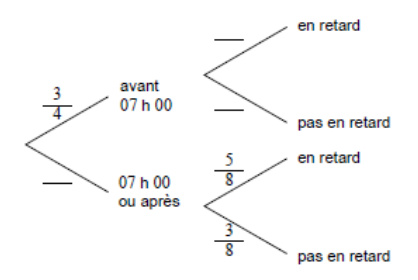
\includegraphics[scale=0.5]{q1_diagram}  

  (b) Trouvez la probabilité que Pablo quitte la maison avant 07 h 00 et qu'il soit en retard.\hspace*{\fill} [2]\par

  (c) Trouvez la probabilité que Pablo soit en retard au travail.\hspace*{\fill} [3]\par

  (d) Sachant que Pablo est en retard au travail,\par
  \hspace{1em}trouvez la probabilité qu’il ait quitté la maison avant 07 h 00.\hspace*{\fill} [3]\par

  (e) Au cours de la semaine prochaine, Pablo se rendra en voiture au travail deux jours.\par
  \hspace{1em}Trouvez la probabilité qu’il soit au moins une fois en retard.\hspace*{\fill} [3]
  
\end{question}

\begin{question}
  \hspace*{\fill} [Note maximale: 5]\par
  \noindent La courbe des effectifs cumulés ci-dessous représente les notes de 100 étudiants.\par

  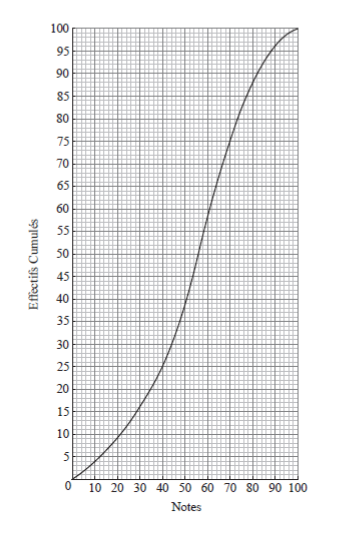
\includegraphics[scale=0.7]{courbe_de_notes}  

  (a) Trouvez la note médianne.\hspace*{\fill} [2]\par
  (b) Trouvez l'intervalle interquartile.\hspace*{\fill} [3]\par
  
\end{question}

\begin{question}
  \hspace*{\fill} [Note maximale: 8]\par
  \medskip
  \noindent La variable aléatoire X suit la distribution de probabilité suivante, avec P(X >1) = 0,5.\par

  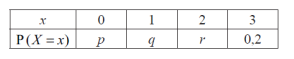
\includegraphics[scale=0.7]{px_table}  

  (a) Trouvez la valeur de r.\hspace*{\fill} [2]\par
  (b) Étant donné que E(X ) =1,4 , trouvez la valeur de p et celle de q. \hspace*{\fill} [6]\par
  
\end{question}
\newpage

\begin{question}
  \hspace*{\fill} [Note maximale: 14]\par
  \medskip
  \noindent Un sac A contient trois boules blanches et quatre boules rouges.\par
  \noindent Deux boules sont choisies au hazard et sans remise.\par
  \medskip
  (a)\par
  \hspace{1em} (i) Copiez et complétez le diagramme en arbre suivant. (N’écrivez rien sur cette page.)\par
  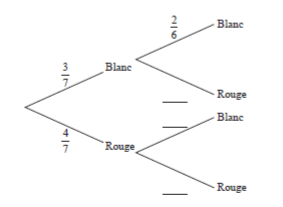
\includegraphics[scale=0.7]{arbre_rb}\par
  \hspace{1em} (ii) Trouvez la probabilité que deux boules blanches soient choisies.\hspace*{\fill} [5]\par
  \medskip  
  \noindent Un sac B contient quatre boules blanches et trois boules rouges. Quand deux boules sont choisies au hasard et sans remise dans le sac B, la probabilité qu’elles soient toutes les deux blanches est $\frac{2}{7}$\par
  \medskip
  \noindent Un dé standard est lancé. Si l’on obtient 1 ou 2, deux boules sont choisies au hasard et sans remise dans le sac A, sinon elles sont choisies dans le sac B.\par
  \medskip
  (b) Trouvez la probabilité que les deux boules soient blanches.\hspace*{\fill} [5]\par
  \medskip
  (c) Étant donné que les deux boules sont blanches,\par
  \hspace{2em}trouvez la probabilité qu’elles aient été choisies dans le sac A.\hspace*{\fill} [4]\par
  
  
\end{question}

\newpage

\begin{question}
  \hspace*{\fill} [Note maximale: 5]\par
  \medskip

  \noindent Une scientifique étudie 100 poissons femelles et 100 poissons mâles. Elle mesure 
  leur longueur (arrondie au centimètre le plus proche). Les résultats sont donnés dans
  les diagrammes à boîtes et moustache suivants.\par
  \medskip

  \noindent Poissons femelles\par
  \medskip

  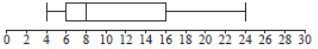
\includegraphics[scale=0.7]{poissons_femelles}\par  
  \medskip

  \noindent Poissons mâles\par
  \medskip

  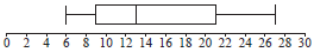
\includegraphics[scale=0.7]{poissons_males}\par  
  \medskip

  (a) Trouvez l’étendue des longueurs de tous les 200 poissons.\hspace*{\fill} [3]\par
  \medskip

  \noindent Quatre courbes de fréquence cumulée sont représentées ci-dessous.\par
  \medskip

  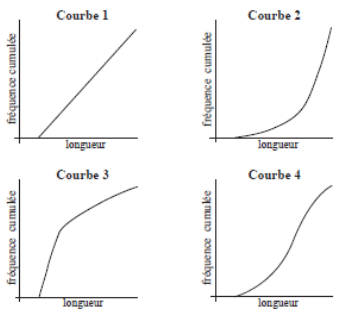
\includegraphics[scale=0.7]{courbe_1_a_4}\par  
  \medskip
  (b) Quelle courbe représente le mieux les longueurs des poissons femelles ?\hspace*{\fill} [2]\par  
\end{question}

\newpage

\begin{question}
  \hspace*{\fill} [Note maximale: 7]\par
  \medskip

  \noindent Le diagramme de Venn ci-dessous représente les événements A et B où $P(A) = 0,3$ ,\par
  
  \noindent $P(AB) = 0,6 $ et $P(AB) = 0,1$. Les valeurs m , n , p et q sont des probabilités. \par

  \medskip

  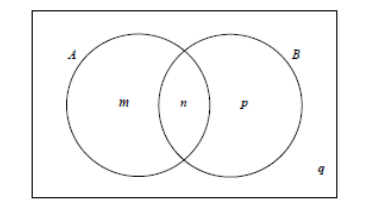
\includegraphics[scale=0.7]{venn_a_b}\par  
  \medskip
  

  (a)\par
  \hspace{2em}(i)  Donnez la valeur de n .\par
  \hspace{2em}(ii) Trouvez la valeur de m , de p et de q .\hspace*{\fill} [4]\par
  
  \medskip

  
  (b) Trouvez $P(B)$.\hspace*{\fill} [2]\par
  
\end{question}


\end{document}
